\chapter{Wellen, quantisierte Moden und Erzeugungsoperatoren}

\section{Wellen, Felder und komplexe Exponentialfunktionen}

Die Quantenfeldtheorie ist das grundlegende Werkzeug der Teilchenphysik. Bevor wir auch nur eine elementare Einführung in Quantenfelder geben, lohnt es sich, die mathematischen Tatsachen zusammenzustellen, die Wellen mit Teilchen verbinden. Eine Welle ist bereits eine Feldkonfiguration: Ein Feld nimmt an verschiedenen Raumpunkten unterschiedliche Werte an, und bei einer Welle schwingen diese Werte und breiten sich aus. Die Quantenmechanik stellt die Verbindung zwischen solchen Wellen und Teilchen her.

Quantenmechanik und spezielle Relativitätstheorie werden hier als bekannt vorausgesetzt. Es geht zunächst darum, die für die Teilchenphysik benötigten Grundlagen zu wiederholen, nicht darum, einen Kurs in einem dieser Fächer zu ersetzen.

Eine Exponentialfunktion ist durch proportionales Wachstum gekennzeichnet. Wenn
\begin{equation}
f(x)=e^{\alpha x},
\end{equation}
dann gilt
\begin{equation}
\frac{df}{dx}=\alpha f.
\end{equation}
Über ein kleines Intervall hinweg ist der Zuwachs proportional zu der bereits vorhandenen Menge. Eine Population, die in einer Petrischale wächst, veranschaulicht das auf vertraute Weise: Je mehr Organismen vorhanden sind, desto mehr können sich fortpflanzen, sodass die Zuwachsrate proportional zur Population selbst ist. Eine Multiplikation von \(e^{\alpha x}\) mit einer konstanten Gesamtgröße ändert an dieser definierenden Eigenschaft nichts.

Sinus und Kosinus schwingen, statt zu wachsen. Es handelt sich um dieselbe Kurve, um ein Viertel einer Periode gegeneinander verschoben, und beim Ableiten gehen sie ineinander über:
\begin{align}
\frac{d}{dx}\sin(kx)&=k\cos(kx),\\
\frac{d}{dx}\cos(kx)&=-k\sin(kx).
\end{align}
Keine der beiden Funktionen ist für sich allein eine Exponentialfunktion, denn ihre Ableitung ist proportional zur jeweils anderen Funktion. Die komplexe Kombination besitzt dagegen die Eigenschaft einer Exponentialfunktion. Mit \(i^2=-1\) gilt:
\begin{align}
\frac{d}{dx}\bigl(\cos(kx)+i\sin(kx)\bigr)
&=-k\sin(kx)+ik\cos(kx)\\
&=ik\bigl(\cos(kx)+i\sin(kx)\bigr).
\end{align}
Daher
\begin{equation}
e^{ikx}=\cos(kx)+i\sin(kx).
\end{equation}
Diese Identität begegnet uns immer wieder, weil sich wellenartige Schwingungen durch Sinus und Kosinus beschreiben lassen. Ist \(x\) eine Ortskoordinate, schwingt die Funktion im Raum. Ist das Argument die Zeit, schwingt sie zeitlich.

\section{Frequenz, Wellenlänge und Photonenimpuls}

Die gewöhnliche Frequenz \(f\) gibt die Anzahl vollständiger Perioden pro Sekunde an. Eine Periode ist eine vollständige Schwingung. Die Kreisfrequenz beschreibt dieselbe Bewegung in Radiant pro Sekunde:
\begin{equation}
\omega=2\pi f.
\end{equation}
Beide Schreibweisen beschreiben dieselbe Frequenz. Man wechselt zwischen ihnen, um unnötige Faktoren von \(2\pi\) aus einer Rechnung herauszuhalten; ganz verschwinden diese Faktoren allerdings nie.

Die Wellenlänge \(\lambda\) ist die Strecke, die eine vollständige räumliche Periode einnimmt. Breitet sich eine Welle mit der Geschwindigkeit \(v\) aus, dann ergibt das Produkt aus der Strecke pro Periode und der Anzahl der Perioden pro Sekunde ihre Ausbreitungsgeschwindigkeit:
\begin{equation}
\lambda f=v.
\end{equation}
Für Licht im Vakuum gilt \(v=c\), also
\begin{equation}
\lambda f=c.
\end{equation}
Bei einer Schallwelle steht auf der rechten Seite die Schallgeschwindigkeit, bei einer Wasserwelle die entsprechende Ausbreitungsgeschwindigkeit der Wasserwelle. Das Auftreten von \(c\) ist daher eine Aussage über Licht und keine Definition, die für alle Wellen gilt.

In der Quantenmechanik wird die Planck-Konstante in zwei Schreibweisen eingeführt:
\begin{equation}
\hbar=\frac{h}{2\pi}.
\end{equation}
Beim Wechsel von \(h\) zu \(\hbar\) werden lediglich Faktoren von \(2\pi\) von einer Gleichung in eine andere verschoben.

Die Zahlenwerte dimensionsbehafteter Konstanten hängen von den verwendeten Einheiten ab. Meter, Sekunden und Kilogramm sind am menschlichen Maßstab orientierte Konventionen, die für gewöhnliche Längen und Zeiten praktisch sind. Traditionelle Maße in der Größenordnung einer Armlänge waren für Stoffe oder Seile nützlich; unabhängig davon, wie genau es historisch zur Festlegung des Meters kam, gibt es kein fundamentales Prinzip, das gerade diese menschliche Größenskala auszeichnet. In SI-Einheiten gilt:
\begin{equation}
\begin{aligned}
h &\simeq 6.6\times10^{-34}\ \mathrm{J\,s},
&\hbar &\simeq 1.1\times10^{-34}\ \mathrm{J\,s},\\
c &\simeq 3\times10^8\ \mathrm{m\,s^{-1}}.
\end{aligned}
\end{equation}
Diese Zahlen sollen vor allem ihre Größenordnung in den gebräuchlichen Einheiten veranschaulichen: Die Planck-Konstante ist außerordentlich klein, die Lichtgeschwindigkeit außerordentlich groß.

Ein Quant einer Mode besitzt die Energie
\begin{equation}
E_{\text{one quantum}}=\hbar\omega=hf.
\end{equation}
Das ist die Energie eines einzelnen Photons, nicht die Gesamtenergie einer beliebigen klassischen elektromagnetischen Welle. Sichtbares Licht hat eine Frequenz in der Größenordnung von \(10^{15}\) Perioden pro Sekunde, sodass ein typisches optisches Photon eine Energie in der Größenordnung von
\begin{equation}
E_\gamma\sim 10^{-19}\ \mathrm{J}.
\end{equation}
besitzt. Selbst eine so schnelle optische Schwingung entspricht pro Quant einer sehr kleinen Energie, weil \(h\) so klein ist. Eine makroskopische Menge optischer Energie enthält daher eine enorm große Anzahl von Photonen.

Energie und Impuls verdienen besondere Aufmerksamkeit, denn beide Größen sind erhalten. Sie dienen als nützliche Buchhaltungsgrößen: Die Gesamtenergie und der Gesamtimpuls, die in einen Prozess hineingehen, müssen mit der Gesamtenergie und dem Gesamtimpuls übereinstimmen, die ihn verlassen. Der Impuls ist ein Vektor und zeigt in Bewegungsrichtung. Für ein Teilchen, das sich viel langsamer als Licht bewegt, gilt
\begin{equation}
\vec p=m\vec v.
\end{equation}

Betrachten wir nun elektromagnetische Strahlung, die in eine Richtung gebündelt ist, statt sich in viele Richtungen auszubreiten. Ihr Impuls zeigt entlang des Strahls. Die nichtrelativistische Formel lässt sich nicht auf ein Photon anwenden, denn \(m\) bezeichnet die Ruhemasse, und ein Photon hat keine Ruhemasse. Es gibt jedoch eine nützliche Dimensionsstütze. Weist man dem Photon \(E/c^2\) einmal \emph{unpassenderweise} wie eine Masse zu und setzt dann \(v=c\) ein, erhält man
\begin{equation}
mv\longrightarrow \frac{E}{c^2}c=\frac{E}{c}.
\end{equation}
Dieses Vorgehen liefert zufällig das richtige Ergebnis und die richtigen Einheiten. Es ist aber kein zulässiges Argument dafür, dass ein Photon die Ruhemasse \(E/c^2\) besitzt. Die tatsächliche relativistische Aussage für gebündelte Strahlung lautet
\begin{equation}
|\vec p|=\frac{E}{c}.
\end{equation}
Die Gleichung gibt den Betrag an. Die Richtung ist die Ausbreitungsrichtung der Strahlung.

Für ein einzelnes Photon gilt
\begin{align}
|\vec p_\gamma|
&=\frac{E_\gamma}{c}
=\frac{hf}{c}.
\end{align}
Für Licht gilt
\begin{equation}
\lambda f=c,
\qquad
\frac{f}{c}=\frac{1}{\lambda},
\end{equation}
und daher
\begin{equation}
|\vec p_\gamma|=\frac{hf}{c}=\frac{h}{\lambda}.
\end{equation}

\begin{figure}[t]\centering
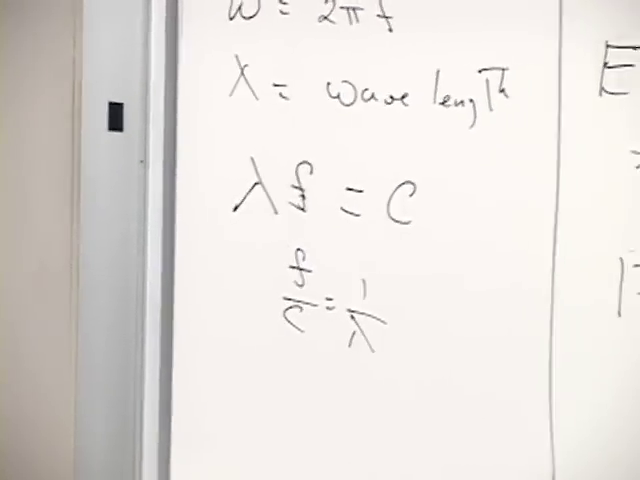
\includegraphics[width=0.56\textwidth]{lecture_02_figure_02.png}\caption{Für Licht gelten \(\lambda f=c\) und \(f/c=1/\lambda\), die Beziehungen, aus denen \(|\vec p_\gamma|=h/\lambda\) folgt.}\lectureframe{00:21:39}\end{figure}

Je kürzer die Wellenlänge, desto größer der Photonenimpuls. Das ist eine der wichtigsten quantenmechanischen Tatsachen für die Teilchenphysik. Um ein kleines Objekt zu untersuchen, braucht man eine Sonde mit kurzer Wellenlänge; der Preis dafür ist ein großer Impuls.

\begin{classroomqa}\lecturetimestamp{00:22:23}\audiencequestion{Ist \(E=\hbar\omega\) fundamental oder lässt es sich aus einem tiefer liegenden Prinzip herleiten?}\lecturerresponse{Es folgt aus der Quantenmechanik des harmonischen Oszillators. Dieses Ergebnis wird hier verwendet, ohne den Beweis zu wiederholen; die weiter unten entwickelte Beschreibung durch Oszillatoren liefert den tieferen Zusammenhang.}\end{classroomqa}


\section{Wellenamplitude und Photonenzahl}

\begin{classroomqa}\lecturetimestamp{00:23:10}\audiencequestion{Was bedeutet die Amplitude einer Welle in der Sprache der Photonen?}\lecturerresponse{Vergleichen wir zwei Wellen mit derselben Wellenlänge und Frequenz, aber unterschiedlicher Amplitude, zum Beispiel \(\sin(kx)\) und \(A\sin(kx)\). Klassisch ist die Energie in einem festen Raumbereich proportional zum Quadrat der Amplitude. Quantenmechanisch besitzt eine Mode mit \(n\) Photonen die Energie \(n\hbar\omega\). Bei fester Frequenz, festem Raumbereich und fester Normierung wächst die Amplitude daher größenordnungsmäßig wie \(\sqrt n\).}\end{classroomqa}

Die beiden Wellen haben dasselbe Schwingungsmuster. Eine ist lediglich stärker als die andere.\footnote{Die schematische Darstellung orientiert sich am Wellenvergleich bei 00:23:47--00:24:28.}

\begin{figure}[t]\centering
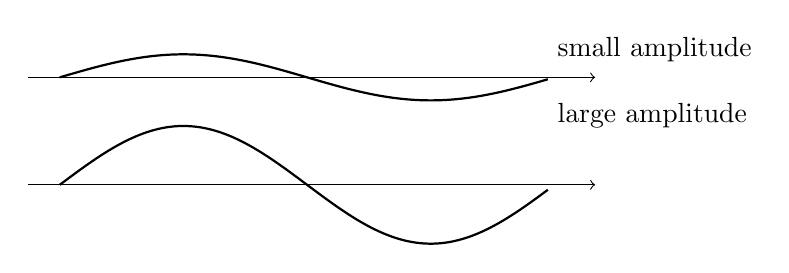
\begin{tikzpicture}[x=1cm,y=0.65cm]
\draw[->] (-0.4,0) -- (6.8,0);
\draw[->] (-0.4,-2.1) -- (6.8,-2.1);
\draw[thick] plot[domain=0:6.2,samples=120] (\x,{0.45*sin(\x r)});
\draw[thick] plot[domain=0:6.2,samples=120] (\x,{-2.1+1.15*sin(\x r)});
\draw (6.2,0.55) node[right]{small amplitude};
\draw (6.2,-0.75) node[right]{large amplitude};
\end{tikzpicture}\caption{Wellen mit gleicher Wellenlänge und Frequenz, aber unterschiedlichen Amplituden.}\end{figure}

Für eine feste Wellenmenge gilt:
\begin{equation}
E_{\text{wave}}\propto A^2.
\end{equation}
Bei einer elektromagnetischen Welle ist das die vertraute Aussage, dass die Feldenergie proportional zum Quadrat der Feldstärke ist. Enthält dieselbe Mode \(n\) Photonen, gilt
\begin{equation}
E_{\text{wave}}=n\hbar\omega.
\end{equation}
Folglich gilt bei festgehaltener Mode, Frequenz, Normierung und festem Raumbereich:
\begin{equation}
A^2\propto n\hbar\omega,
\qquad
A\propto\sqrt n\quad\text{at fixed }\omega.
\end{equation}
Eine exakte Normierung wird hier nicht behauptet. Es kommt darauf an, welche Wellenmenge berücksichtigt wird: Verdoppelt man die Länge einer ansonsten gleichförmigen Welle, ändert sich ihre Gesamtenergie, ohne dass sich die lokale Amplitude ändert. Die Proportionalität lässt sich daher für einen festen Raumbereich verstehen, etwa für eine Wellenlänge.

Dabei ist noch eine spezifisch quantenmechanische Einschränkung zu beachten. Amplitude und Phase können nicht beide exakt wie klassische Größen festgelegt werden. Die Frage ``Wie groß ist die Amplitude eines Photons?'' ist daher mehrdeutig, wenn sie auf ein vollkommen scharf bestimmtes klassisches Feld abzielt. Setzt man dennoch \(n=1\), erhält man eine sinnvolle Größenordnung.

\begin{classroomqa}\lecturetimestamp{00:28:25}\audiencequestion{Gibt die vertikale Auslenkung in einer Zeichnung einer elektromagnetischen Welle die Position des Photons im Raum an?}\lecturerresponse{Nein. Die Ausbreitungsachse ist räumlich, während die vertikale Koordinate den Wert des elektrischen oder magnetischen Feldes darstellt. Der Impuls zeigt entlang der Ausbreitungsachse, nicht in Richtung der eingezeichneten Feldamplitude.}\end{classroomqa}

Die Welle kann sich in jede beliebige Raumrichtung ausbreiten, doch die vertraute Sinuskurve verwendet nur ihre horizontale Achse als Ortskoordinate. Die andere eingezeichnete Richtung gibt die Feldstärke an.

\begin{classroomqa}\lecturetimestamp{00:29:37}\audiencequestion{Wird die angegebene Photonenzahl innerhalb einer Wellenlänge oder einer Periode der Welle gezählt?}\lecturerresponse{Man kann einen festen Raumbereich wählen, zum Beispiel eine Wellenlänge. Deshalb gilt nur eine Proportionalität: Die Gesamtenergie und die Photonenzahl hängen auch davon ab, wie viel von der Welle einbezogen wird. Zwei, drei oder vier Wellenlängen enthalten bei gleicher Amplitude entsprechend mehr Energie als eine Wellenlänge.}\end{classroomqa}

\begin{classroomqa}\lecturetimestamp{00:30:17}\audiencequestion{Ist die Amplitude eines einzelnen Photons bedeutungslos?}\lecturerresponse{Sie ist nur als Größenordnungsaussage sinnvoll, die man erhält, indem man \(n=1\) setzt. Bei einer elektromagnetischen Mode spielen Informationen über das elektrische und das magnetische Feld eine den konjugierten Orts- und Impulsinformationen analoge Rolle. Die quantenmechanische Unschärfe begrenzt daher, wie genau sich eine klassische Amplitude festlegen lässt. Die Größenordnungsbeziehung bleibt nützlich.}\end{classroomqa}

Diese Fragen führen bereits zur Quantenfeldtheorie, in der sich die Beziehung zwischen Feldvariablen und Teilchenzahl präzise formulieren lässt. Für den Moment reichen die Proportionalitäten aus.

\section{Allgemeine Quantenbeziehungen und langsame Materiewellen}

Manche der für Photonen eingeführten Formeln gelten viel allgemeiner, andere dagegen nicht. Bevor wir uns den Elektronen zuwenden, lohnt es sich, die Gültigkeitsbereiche zu ordnen.

\begin{figure}[t]\centering
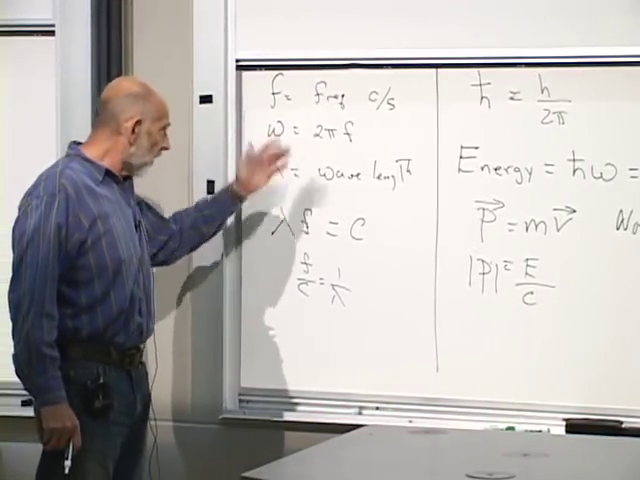
\includegraphics[width=0.82\textwidth]{lecture_02_figure_03.png}\caption{Wellendefinitionen sowie die Impulsbeziehungen für Photonen und nichtrelativistische Teilchen im Vergleich ihrer Gültigkeitsbereiche.}\lectureframe{00:31:52}\end{figure}

Die Definitionen von \(f\), \(\omega=2\pi f\) und \(\lambda\) gelten allgemein. Auch die Quantenbeziehung
\begin{equation}
E=\hbar\omega=hf
\end{equation}
ist in der vorliegenden Diskussion allgemein gültig. Formeln mit \(c\), etwa \(\lambda f=c\) und \(|\vec p|=E/c\), gelten dagegen für Wellen, die sich mit Lichtgeschwindigkeit ausbreiten. Die Formel \(\vec p=m\vec v\) gilt für Teilchen, die sich viel langsamer als Licht bewegen. Für relativistische Bewegungen zwischen diesen Grenzfällen wäre eine Interpolation erforderlich, die wir vorerst nicht benötigen.

Die Impuls--Wellenlängen-Beziehung gilt auch über das Photonbeispiel hinaus:
\begin{equation}
p=\frac{h}{\lambda}.
\end{equation}
Hier bezeichnet \(p\) den Betrag, wenn \(\lambda\) als positive Wellenlänge genommen wird; die Richtung lässt sich gesondert angeben.

\begin{figure}[t]\centering
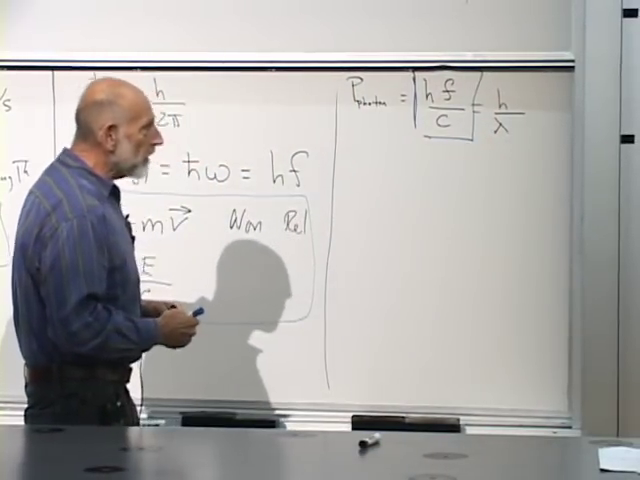
\includegraphics[width=0.74\textwidth]{lecture_02_figure_04.png}\caption{Photonenimpuls \(|\vec p_\gamma|=hf/c=h/\lambda\) als Ausgangspunkt für die allgemeine de-Broglie-Beziehung.}\lectureframe{00:33:32}\end{figure}

Mit einem Elektron, einem Atomkern und sogar einer Bowlingkugel lässt sich eine Welle verknüpfen. Die Interferenz von Elektronen ist eine Erscheinungsform dieser Tatsache. Schreiben wir die Elektronenwelle als \(\psi\). Was tritt bei einem langsam bewegten Elektron an die Stelle von \(\lambda f=c\)? Es fehlt noch die nichtrelativistische Beziehung zwischen Energie und Impuls.

Wir beginnen mit kinetischer Energie und Impuls:
\begin{align}
E&=\frac12 mv^2,\\
p&=mv,
\qquad
v=\frac{p}{m}.
\end{align}
Setzt man die letzte Beziehung in die erste ein, erhält man
\begin{align}
E
&=\frac12m\left(\frac{p}{m}\right)^2\\
&=\frac{p^2}{2m}.
\end{align}
In \(\frac12 mv^2\) steht die Masse im Zähler, in \(p^2/(2m)\) im Nenner. Diese Anordnung lässt sich leicht verwechseln und bei Bedarf einfach erneut herleiten.

Verwenden wir nun die allgemeinen Quantenbeziehungen
\begin{equation}
E=hf,
\qquad
p=\frac{h}{\lambda}.
\end{equation}
Für ein einzelnes langsames Teilchen gilt
\begin{align}
hf
&=\frac{p^2}{2m}\\
&=\frac{1}{2m}\left(\frac{h}{\lambda}\right)^2\\
&=\frac{h^2}{2m\lambda^2}.
\end{align}
Division durch \(h\) ergibt
\begin{equation}
f=\frac{h}{2m\lambda^2}.
\end{equation}

\begin{figure}[t]\centering
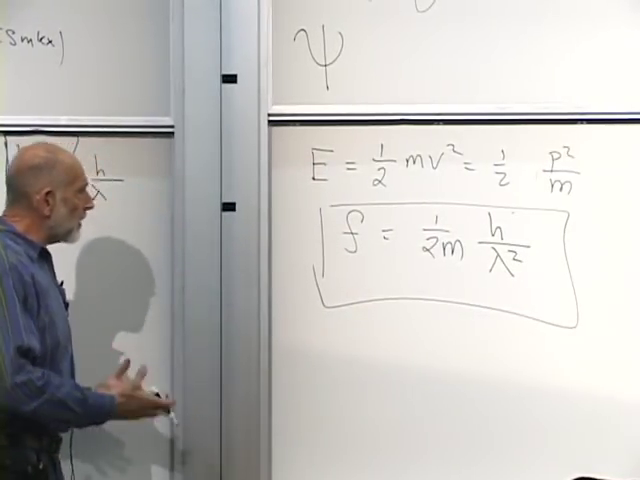
\includegraphics[width=0.64\textwidth]{lecture_02_figure_05.png}\caption{Für ein langsames Teilchen führen \(E=p^2/(2m)\) und \(p=h/\lambda\) auf \(f=h/(2m\lambda^2)\).}\lectureframe{00:37:47}\end{figure}

Für Licht gilt
\begin{equation}
f\propto\frac{1}{\lambda},
\end{equation}
während für langsame Materie gilt
\begin{equation}
f\propto\frac{1}{\lambda^2}.
\end{equation}
Die zweite Beziehung muss man nicht isoliert auswendig lernen. Sie lässt sich stets aus \(E=p^2/(2m)\), \(E=hf\) und \(p=h/\lambda\) rekonstruieren. Für ein langsam bewegtes Elektron in einem Atom gibt sie die Frequenz der zugehörigen Schr\"odinger-Welle an.

\begin{classroomqa}\lecturetimestamp{00:38:35}\audiencequestion{Gilt die nichtrelativistische Frequenz--Wellenlängen-Beziehung auch für andere Teilchen als Elektronen?}\lecturerresponse{Ja. Sie gilt für jedes Teilchen, das sich viel langsamer als Licht bewegt. Die relativistische Interpolation zwischen dem langsamen und dem lichtartigen Grenzfall ist ein eigenes Thema.}\end{classroomqa}

\begin{classroomqa}\lecturetimestamp{00:38:55}\audiencequestion{Welche Beziehung gilt für ein Neutrino?}\lecturerresponse{Das hängt von der Geschwindigkeit des Neutrinos ab. Die meisten Neutrinos, denen man in der Natur begegnet, bewegen sich sehr nahe an der Lichtgeschwindigkeit, sodass die lichtartige Beziehung eine gute Näherung ist. Ein Neutrino, das sich viel langsamer als Licht bewegt, würde dagegen der nichtrelativistischen Beziehung folgen.}\end{classroomqa}

\editorialnote{Ein kurzer Wortwechsel mit dem Publikum unmittelbar nach der Frage zum Neutrino dreht sich um Amplituden, Quanten und unterschiedliche Elektronenwellenlängen; sein Wortlaut ist jedoch zu stark beschädigt, um ihn zuverlässig wiederherzustellen. In der erhaltenen Antwort wird die allgemeine Beziehung zwischen Amplituden und Quanten unterschiedlicher Wellenlängen auf später verschoben.}

\begin{classroomqa}\lecturetimestamp{00:39:56}\audiencequestion{Ist ein Elektron aus einem \(20\,\mathrm{keV}\)-Beschleuniger langsam oder relativistisch?}\lecturerresponse{Es wird als langsam behandelt. In Einheiten mit \(c=1\) lassen sich Masse, Energie und Impuls in denselben Einheiten ausdrücken. Die Ruheenergieskala des Elektrons beträgt ungefähr \(0.5\,\mathrm{MeV}\), während \(20\,\mathrm{keV}\) viel kleiner ist. Gleichwertig dazu lautet das nichtrelativistische Impulskriterium \(p\ll mc\).}\end{classroomqa}

Der Energievergleich im Beispiel lautet
\begin{equation}
K=20\,\mathrm{keV}\ll m_ec^2\simeq0.5\,\mathrm{MeV}.
\end{equation}
\editorialnote{In der Passage bei 00:39:56--00:41:40 wird \(20\,\mathrm{keV}\) als Beschleunigerenergie eingeführt; das relativistische Kriterium wird anschließend als Vergleich des Impulses mit der Ruhemasse formuliert. Wenn man die Kriterien für kinetische Energie und Impuls getrennt angibt, setzt man die genannte Energie nicht mit einem Impuls gleich und bewahrt zugleich die Aussage, dass das Teilchen nichtrelativistisch ist.}

\section{Phasengeschwindigkeit, Gruppengeschwindigkeit und Dispersion}

\begin{classroomqa}\lecturetimestamp{00:41:46}\audiencequestion{Kann man die Geschwindigkeit einer Elektronenwelle bestimmen, indem man Frequenz und Wellenlänge multipliziert?}\lecturerresponse{Das ergibt die Phasengeschwindigkeit, nicht die dem Elektron zugeordnete Geschwindigkeit. Ein lokalisiertes Wellenpaket hat sowohl eine Phasengeschwindigkeit, die die Bewegung seiner inneren Wellenberge und -täler beschreibt, als auch eine Gruppengeschwindigkeit, die die Bewegung der Einhüllenden beschreibt. Die Gruppengeschwindigkeit wird mit der Bewegung des Teilchens identifiziert.}\end{classroomqa}

Ein Wellenpaket sieht lokal wie ein Sinus oder Kosinus aus, ist aber durch eine Einhüllende begrenzt. Bei seiner Ausbreitung müssen sich die Einhüllende und die Wellenberge in ihr nicht mit derselben Geschwindigkeit bewegen.\footnote{Die schematische Darstellung orientiert sich an der Erörterung von Wellenpaketen bei 00:42:34--00:44:11.}

\begin{figure}[t]\centering
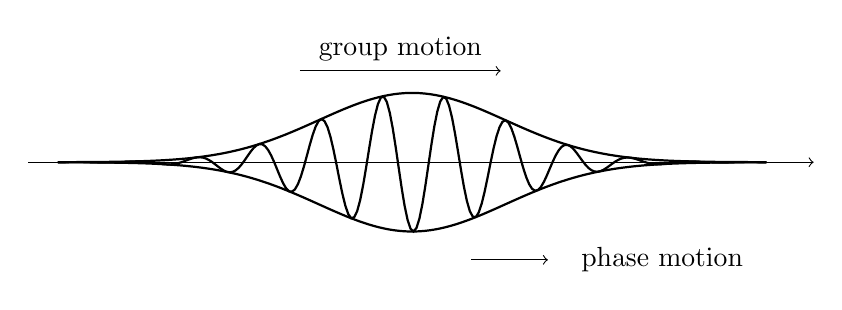
\begin{tikzpicture}[x=0.75cm,y=0.8cm]
\draw[->] (-0.5,0) -- (12.8,0);
\draw[thick] plot[domain=0:12,samples=140] (\x,{1.10*exp(-0.20*(\x-6)^2)});
\draw[thick] plot[domain=0:12,samples=140] (\x,{-1.10*exp(-0.20*(\x-6)^2)});
\draw[thick] plot[domain=0:12,samples=240] (\x,{1.10*exp(-0.20*(\x-6)^2)*sin(6*\x r)});
\draw[->] (4.1,1.45) -- (7.5,1.45);
\draw (5.8,1.8) node{group motion};
\draw[->] (7.0,-1.55) -- (8.3,-1.55);
\draw (8.7,-1.55) node[right]{phase motion};
\end{tikzpicture}\caption{Ein lokalisiertes Wellenpaket, dessen Einhüllende und innere Phase sich im Allgemeinen mit unterschiedlichen Geschwindigkeiten bewegen.}\end{figure}

Die Phasengeschwindigkeit ist die Geschwindigkeit der Wellenberge, Wellentäler und anderer Phasen gleicher Phase einer monochromatischen Komponente. Für die nichtrelativistische Dispersionsrelation gilt
\begin{equation}
v_\phi=f\lambda=\frac{h}{2m\lambda}.
\end{equation}
Sie hängt von der Wellenlänge ab. Komponenten mit unterschiedlichen Wellenlängen haben daher unterschiedliche Phasengeschwindigkeiten, sodass sich die Wellenberge durch das Paket bewegen und das Paket dispersieren kann. Die Gruppengeschwindigkeit ist die Geschwindigkeit des Pakets als Ganzes; sie wird mit der des Teilchens identifiziert.

Es gibt einen einfachen Sonderfall. Bewegen sich alle Wellenlängenkomponenten mit derselben Geschwindigkeit, stimmen Phasen- und Gruppengeschwindigkeit überein. Licht im Vakuum besitzt diese Eigenschaft: Jede Wellenlänge breitet sich mit \(c\) aus. Für langsame Teilchen gilt diese Beziehung nicht; dort ändert sich \(f\lambda\) mit \(\lambda\).

Die Gleichung
\begin{equation}
f=\frac{h}{2m\lambda^2}
\end{equation}
ist die freie Schr\"odinger-Gleichung in leicht verkleideter Form. Die Frequenz legt die zeitliche Abhängigkeit einer ebenen Welle fest, die Wellenlänge ihre räumliche Abhängigkeit, und die Schr\"odinger-Gleichung verknüpft beides. Umgekehrt ergibt das Einsetzen einer Welle mit fester Frequenz und Wellenlänge in die freie Schr\"odinger-Gleichung wieder diese Dispersionsrelation.

\begin{classroomqa}\lecturetimestamp{00:47:02}\audiencequestion{Kann die Phasengeschwindigkeit größer als die Lichtgeschwindigkeit sein?}\lecturerresponse{Ja. Die Phasengeschwindigkeit überträgt keine Information. Information und das lokalisierte Wellenpaket breiten sich mit der Gruppengeschwindigkeit aus; eine überlichtschnelle Phasengeschwindigkeit ermöglicht daher keine überlichtschnelle Signalübertragung.}\end{classroomqa}

\section{Endlicher Raum und diskreter Impuls}

Letztlich interessieren uns Wellen im unendlichen Raum, doch ein endliches System ist der sicherere Ausgangspunkt. Ein Computer kann Unendlichkeit nicht unmittelbar speichern oder verarbeiten. Zunächst formuliert man die Gleichungen für ein endliches System und bildet erst danach den Grenzfall, in dem dessen Größe beliebig groß wird. Diese Vorgehensweise ist in der gesamten Quantenmechanik, Quantenfeldtheorie und Teilchenphysik nützlich.

Wenn man mit einer Raumdimension beginnt, geht nichts Wesentliches verloren. Die Welle könnte sich auf einer Geigensaite, einem geschüttelten Seil oder in einer abstrakten eindimensionalen Welt befinden. Das naheliegendste endliche System ist ein Abschnitt der Länge \(L\) mit reflektierenden Enden. Eine Welle läuft zu einem Ende, wird reflektiert und läuft zurück. Das ist eine vollkommen zulässige reflektierende Randbedingung, hat aber einen Nachteil: Der Impuls ist innerhalb des Wellensystems nicht erhalten. Eine nach rechts laufende Welle trägt nach rechts gerichteten Impuls; nach der Reflexion trägt sie nach links gerichteten Impuls. Die Randfläche hat den Impuls übertragen und die Differenz aufgenommen.

Die Impulsumkehr an einem reflektierenden Ende lässt sich schematisch darstellen.\footnote{Die schematische Darstellung veranschaulicht die Argumentation zur reflektierenden Randbedingung bei 00:49:24--00:51:08.}

\begin{figure}[t]\centering
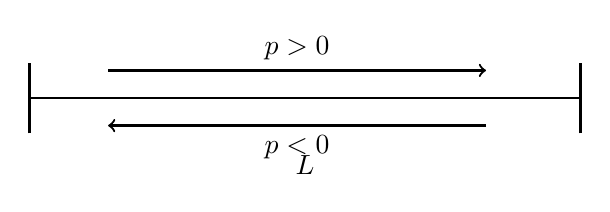
\begin{tikzpicture}[x=1cm,y=1cm]
\draw[thick] (0,0) -- (7,0);
\draw[very thick] (0,-0.45) -- (0,0.45);
\draw[very thick] (7,-0.45) -- (7,0.45);
\draw[->,thick] (1.0,0.35) -- (5.8,0.35) node[midway,above]{\(p>0\)};
\draw[->,thick] (5.8,-0.35) -- (1.0,-0.35) node[midway,below]{\(p<0\)};
\draw (3.5,-0.85) node{\(L\)};
\end{tikzpicture}\caption{Die Reflexion an den Enden eines endlichen Abschnitts kehrt den Impuls einer laufenden Welle um.}\end{figure}

Es gibt eine andere Möglichkeit, das System endlich zu machen und dabei den Impuls zu erhalten. Dazu identifiziert man die beiden Endpunkte des Abschnitts. Man kann sich das Ergebnis als Kreis vorstellen, doch dafür ist kein buchstäblicher Kreis erforderlich, der in eine zweite Dimension eingebettet ist. Die mathematische Aussage lautet schlicht, dass die Koordinate periodisch ist: Nach einer zurückgelegten Gesamtstrecke von \(L\) kehrt man zum selben Punkt zurück.

\begin{figure}[t]\centering
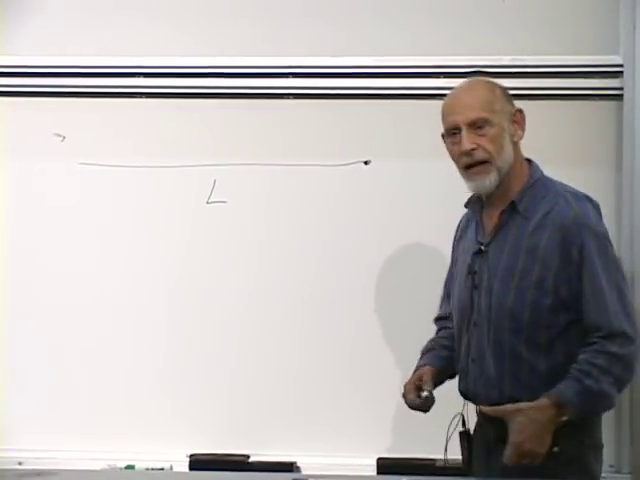
\includegraphics[width=0.72\textwidth]{lecture_02_figure_06.png}\caption{Ein eindimensionaler Weg der Gesamtlänge \(L\) zur Einführung der periodischen Identifikation.}\lectureframe{00:51:21}\end{figure}

Die Identifikation der Endpunkte ist in der folgenden schematischen Darstellung veranschaulicht.\footnote{Die schematische Darstellung orientiert sich an der Erörterung der periodischen Identifikation bei 00:51:09--00:52:37.}

\begin{figure}[t]\centering
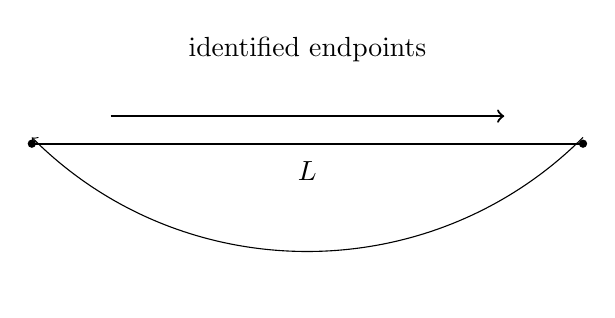
\begin{tikzpicture}[x=1cm,y=1cm]
\draw[thick] (0,0) -- (7,0);
\fill (0,0) circle (1.5pt);
\fill (7,0) circle (1.5pt);
\draw[->,thick] (1.0,0.35) -- (6.0,0.35);
\draw (3.5,-0.35) node{\(L\)};
\draw[->,bend left=45] (7,0.08) to (0,0.08);
\draw (3.5,1.2) node{identified endpoints};
\end{tikzpicture}\caption{Eindimensionaler periodischer Raum, der durch Identifikation der Endpunkte eines Weges der Länge \(L\) entsteht.}\end{figure}

Eine nach rechts laufende Welle erreicht dann den dargestellten Endpunkt, tritt am Anfang wieder ein und läuft weiter nach rechts. Eine nach links laufende Welle setzt ihre Bewegung ebenfalls nach links fort. Es gibt keinen ausgezeichneten Endpunkt, an dem die Welle reflektiert würde, sodass sich der Impuls nicht umkehrt. Der periodische Raum macht das Volumen endlich und erhält den Impuls, hat aber eine wichtige Folge: Die möglichen Impulse sind diskret.

In die Gesamtlänge muss eine ganzzahlige Anzahl von Wellenlängen passen. Für eine nichtkonstante Mode gilt:
\begin{equation}
\lambda_{|N|}=\frac{L}{|N|},
\qquad |N|=1,2,3,\ldots .
\end{equation}
Die Wellenlänge kann also \(L\), \(L/2\), \(L/3\) und so weiter betragen. Eine Wahl wie \(L/\sqrt{2}\) passt nicht: Nach einem Umlauf würde die Welle mit der falschen Phase zurückkehren und nicht mit ihrem Anfangswert übereinstimmen.

Mit \(p=h/\lambda\) beträgt der Impulsbetrag der \(|N|\)-ten nichtkonstanten Mode
\begin{equation}
|p_N|=\frac{|N|h}{L}.
\end{equation}
Um beide Richtungen und die konstante Mode eindeutig zu berücksichtigen, ist es praktisch, die Modenbezeichnung vorzeichenbehaftet zu wählen:
\begin{equation}
p_N=\frac{Nh}{L},
\qquad N=0,\pm1,\pm2,\ldots .
\end{equation}
Positive und negative Werte von \(N\) stehen für entgegengesetzte Ausbreitungsrichtungen. Die Mode \(N=0\) ist konstant und hat den Impuls null; sie besitzt keine endliche Wellenlänge, die man in \(h/\lambda\) einsetzen könnte. Der grundlegende Impulsabstand beträgt daher \(h/L\).

Für ein makroskopisches \(L\) sind sowohl \(h\) als auch \(1/L\) groß, sodass dieser Impulsabstand äußerst klein ist. Die erlaubten Werte liegen dann sehr dicht beieinander und erscheinen nahezu kontinuierlich. Eine Perle, die auf einen kreisförmigen Draht beschränkt ist, besitzt trotzdem genau dieses diskrete Spektrum.

\begin{classroomqa}\lecturetimestamp{00:58:27}\audiencequestion{Wird der Gesamtimpuls der Welle quantisiert oder der Impuls einer einzelnen Periode?}\lecturerresponse{Die Aussage bezieht sich auf den Impuls jedes einzelnen Quants. Jedes Quant besitzt einen der erlaubten diskreten Impulse. Der Gesamtimpuls einer beliebigen Sammlung von Quanten ist daher ebenfalls ein ganzzahliges Vielfaches der Grundeinheit \(h/L\).}\end{classroomqa}

\begin{classroomqa}\lecturetimestamp{00:59:22}\audiencequestion{Warum muss die Welle nach einem Umlauf zu demselben Wert zurückkehren?}\lecturerresponse{Die identifizierten Endpunkte sind derselbe physikalische Punkt, daher muss ein beobachtbares Feld dort denselben Wert haben. Eine Abweichung würde an diesem Punkt einen plötzlichen Sprung des Feldes erfordern. Eine solche Unstetigkeit ist mit hohen Energie- und Impulskosten verbunden; zulässige Feldkonfigurationen sind stetig und periodisch.}\end{classroomqa}

\begin{classroomqa}\lecturetimestamp{01:00:09}\audiencequestion{Was passiert, wenn die Welle in einem Paket lokalisiert ist?}\lecturerresponse{Ein Paket ist eine Fourier-Summe ebener Wellen oder, gleichbedeutend, von Sinus- und Kosinusfunktionen. Im periodischen Raum darf diese Summe nur die diskreten, erlaubten Impulsmoden enthalten. Die Quantisierungsaussage bezieht sich somit auf die Fourier-Komponenten jedes zulässigen Pakets.}\end{classroomqa}

\begin{classroomqa}\lecturetimestamp{01:01:01}\audiencequestion{Gibt es ein Problem, wenn die periodische Länge \(L\) extrem klein wird?}\lecturerresponse{Wenn \(L\) abnimmt, wird der grundlegende Impuls \(h/L\) sehr groß. Bei gewöhnlichen mikroskopischen Längen folgt daraus kein unmittelbarer Widerspruch; für eine Fortsetzung der Konstruktion bis zur Planck-Längenskala dürfte jedoch neue Physik erforderlich sein.}\end{classroomqa}

Nehmen wir nun die Kreisvorstellung wörtlich: Eine Perle bewegt sich auf einem kreisförmigen Draht mit Radius \(r\) und Umfang \(L=2\pi r\). Ihre erlaubten tangentialen Impulse sind
\begin{equation}
p_N=\frac{Nh}{2\pi r}=\frac{N\hbar}{r}.
\end{equation}
Für ein nichtrelativistisches Teilchen auf einer Kreisbahn ist der Drehimpuls \(mvr\). Da in diesem Bereich \(p=mv\) gilt, ist er gleich \(rp\). Der Ausdruck \(mvr\) gilt nicht allgemein relativistisch, denn dann ist \(p\) nicht einfach \(mv\); das Produkt aus Impuls und senkrechtem Abstand bleibt jedoch die richtige Beziehung. In Vektorform lautet sie:\footnote{In der Vorlesung wird zunächst \(L\) für den Drehimpuls verwendet; dann fällt die Überschneidung mit \(L\) für die periodische Länge auf und es wird ein anderes Symbol gewählt. Hier wird durchgehend \(J\) verwendet; siehe 01:03:40--01:05:21.}
\begin{equation}
\vec J=\vec r\times\vec p,
\end{equation}
Bei einer tangentialen Kreisbewegung ist sein Betrag \(J=rp\). Somit gilt
\begin{equation}
J_N=rp_N=N\hbar.
\end{equation}
Der Abstand der linearen Impulse hängt von der Größe des Kreises ab, während die Einheit des Drehimpulses stets \(\hbar\) beträgt. Bei Fermionen gibt es Ausnahmen von der Ganzzahligkeitsregel; darauf gehen wir später ein.

Als Nächstes soll die Beziehung zwischen Feldern, Teilchen und Quanten präziser hergestellt werden. Dafür ist ein kurzer Rückgriff auf die Quantenmechanik von Operatoren und den harmonischen Oszillator nötig.

\section{Wellenmoden und Quantenoperatoren}

Die folgende Quantenmechanik ist notwendigerweise abstrakt und als Wiederholung gedacht. Der harmonische Oszillator ist das entscheidende System, denn eine Welle ist eine Schwingung. An einem festen Punkt ändert sich die Amplitude eines elektrischen Feldes, eines magnetischen Feldes oder einer anderen Welle periodisch mit der Zeit; von einer Frequenz einer Komponente zu sprechen heißt bereits, dass sie schwingt.

Eine allgemeine Welle muss nicht nur eine einzige Wellenlänge haben. Licht verschiedener Farben kann miteinander gemischt werden; umgekehrt kann ein Prisma gemischtes Licht in seine einzelnen Farben zerlegen, wie Newton es bei der Zerlegung weißen Lichts tat. Jede Komponente hat ihre eigene Wellenlänge, Frequenz, Amplitude, Energie und ihren eigenen Impuls. Die gemischte Welle lässt sich somit in Quanten unterschiedlicher Energien und Impulse zerlegen. Jede Wellenlänge legt eine Frequenz fest, und jede Komponente mit bestimmter Frequenz verhält sich wie ein Oszillator. Deshalb ist der harmonische Oszillator der natürliche Baustein eines Feldes und nicht ein beliebiges Quantensystem.

Quantenmechanische Observablen werden durch Operatoren dargestellt. Operatoren lassen sich addieren und multiplizieren, doch anders als bei gewöhnlichen Zahlen muss das Produkt nicht unabhängig von der Reihenfolge sein. Seien \(A\) und \(B\) Darstellungen zweier Eigenschaften eines Systems, die jeweils für sich messbar sein könnten. So könnte \(A\) beispielsweise ein elektrisches Feld und \(B\) ein magnetisches Feld darstellen. Sind die Messwerte die gewöhnlichen Zahlen \(a\) und \(b\), dann gilt
\begin{equation}
ab=ba.
\end{equation}
Ihr numerisches Produkt kann nicht von der Reihenfolge der Multiplikation abhängen. In der Quantenmechanik können die entsprechenden Operatoren dagegen stattdessen \(AB-BA\neq0\) erfüllen.

Auf den ersten Blick scheint das unsinnig. Wenn die Messung des elektrischen Feldes eine Zahl und die des magnetischen Feldes eine andere ergibt, muss das Produkt dieser beiden Zahlen in beiden Reihenfolgen dasselbe Ergebnis liefern. Die Auflösung besteht darin, dass sich zwei Größen nicht gleichzeitig messen lassen, wenn ihre Operatorprodukte von der Reihenfolge abhängen. Das Experiment zur Messung der einen Größe stört die Messung der anderen. Es liegt kein Widerspruch vor, denn die beiden Zahlenwerte lassen sich nicht gemeinsam bestimmen.

Wenn sich zwei Größen gleichzeitig messen lassen, sind ihre Messwerte gewöhnliche Zahlen und kommutieren miteinander. Ob sie gleichzeitig messbar sind, prüft man daher mit dem Kommutator
\begin{equation}
[A,B]=AB-BA.
\end{equation}
Ein verschwindender Kommutator bedeutet, dass die Observablen miteinander verträglich sind; ein von null verschiedener Kommutator bedeutet, dass sich die entsprechenden Messungen gegenseitig stören. Vertauscht man die Einträge, ändert sich das Vorzeichen:
\begin{equation}
[B,A]=-[A,B].
\end{equation}

Bei einem nichtrelativistischen Teilchen kommutieren die drei Ortskomponenten untereinander, und ebenso die drei Impulskomponenten:
\begin{align}
[x,y]&=[y,z]=[z,x]=0,\\
[p_x,p_y]&=[p_y,p_z]=[p_z,p_x]=0.
\end{align}
Alle drei Koordinaten lassen sich gemeinsam festlegen, ebenso alle drei Impulskomponenten. Entsprechende Orts- und Impulskomponenten kommutieren dagegen nicht:
\begin{equation}
[x,p_x]=[y,p_y]=[z,p_z]=i\hbar,
\end{equation}
Gemischte Komponenten wie \([x,p_y]\) verschwinden hingegen. Eine Messung einer Ortskoordinate versetzt den Teilchenimpuls in der dazu konjugierten Richtung in Unruhe. Anders ausgedrückt: Das Produkt der entsprechenden Unsicherheiten von Ort und Impuls wird durch \(\hbar\) bestimmt.

\begin{classroomqa}\lecturetimestamp{01:16:30}\audiencequestion{Ändert sich beim Wechsel von \(x\) zu \(y\) das \(i\) im Kommutator zu \(j\)?}\lecturerresponse{Nein. Das Symbol \(i\) bezeichnet immer die imaginäre Einheit, also die Quadratwurzel aus minus eins. Es ist weder die Bezeichnung eines kartesischen Einheitsvektors noch eines der Quaternionensymbole \(i,j,k\).}\end{classroomqa}

\begin{classroomqa}\lecturetimestamp{01:17:24}\audiencequestion{Bedeutet \(AB-BA\), zuerst \(A\) und dann \(B\) zu messen und anschließend die Messreihenfolge umzukehren?}\lecturerresponse{Nein. Die beiden Terme sind Operator- oder Matrixprodukte in unterschiedlicher algebraischer Reihenfolge. Sie bezeichnen keine wörtliche Abfolge von Messungen. Der Zusammenhang mit nicht miteinander verträglichen Messungen folgt aus der Operatoralgebra; er ist nicht die Definition des Produkts.}\end{classroomqa}

\begin{classroomqa}\lecturetimestamp{01:18:32}\audiencequestion{Gelten diese Kommutatoren von Ort--Impuls unmittelbar auch für ein Photon?}\lecturerresponse{Nicht unmittelbar. Sie gelten in klarer Form für nichtrelativistische Teilchen. Die Position eines Photons lässt sich schwieriger definieren; die analoge Aussage erfordert daher mehr Sorgfalt und wird hier nicht benötigt.}\end{classroomqa}

\section{Der quantenmechanische harmonische Oszillator}

Ein Gewicht an einer Feder, eine Schallwelle und eine Lichtwelle sind Beispiele für Schwingungen. Jeder ideale harmonische Oszillator hat eine Frequenz. Bei einer Feder ist eine volle Periode nicht einfach die Zeit, bis das Gewicht wieder dieselbe Position erreicht; es muss diese Position auch in derselben Richtung durchlaufen. Die Zahl der vollständigen Perioden pro Sekunde ist \(f\), und es gilt \(\omega=2\pi f\).

Klassisch kann ein idealer Oszillator jede nichtnegative Energie haben. Ein sanfter Stoß verleiht ihm wenig Energie, ein kräftigerer mehr. Eine reale Feder würde irgendwann brechen oder schmelzen, doch die mathematische Idealisierung besitzt ein kontinuierliches Spektrum positiver Energien. Beim Quantenoszillator ist das anders: Seine erlaubten Energien bilden eine diskrete, gleichmäßig abgestufte Leiter. Wählt man den Energienullpunkt so, dass das niedrigste Niveau null heißt, gilt
\begin{equation}
E_n=n\hbar\omega,
\qquad n=0,1,2,\ldots .
\end{equation}
Die gleichmäßig abgestuften Niveaus lassen sich wie folgt veranschaulichen.\footnote{Das Energieniveauschema folgt der Tafelbesprechung bei 01:21:20--01:23:56.}

\begin{figure}[t]\centering
\begin{tikzpicture}[x=1cm,y=0.9cm]
\draw[->] (0,0) -- (0,5.35);
\draw (0,5.5) node[above]{energy};
\foreach \y/\lab in {0.6/{0},1.6/{\hbar\omega},2.6/{2\hbar\omega},3.6/{3\hbar\omega},4.6/{n\hbar\omega}}
{
  \draw[thick] (0.2,\y) -- (2.2,\y);
  \draw (-0.25,\y) node[left]{\(\lab\)};
}
\draw[->,thick] (2.8,0.68) -- (2.8,1.52);
\draw (3.2,1.1) node[right]{\(a_+\)};
\draw[->,thick] (3.7,1.52) -- (3.7,0.68);
\draw (4.1,1.1) node[right]{\(a_-\)};
\end{tikzpicture}\caption{Gleichmäßig abgestufte Oszillatorniveaus gemäß der Konvention \(E_n=n\hbar\omega\).}\end{figure}

Der Abstand \(\hbar\omega\) ist dieselbe Energie, die zuvor einem Photon mit der Kreisfrequenz \(\omega\) zugeordnet wurde. Der Wert \(2\hbar\omega\) könnte die Energie eines einzelnen Quants eines Oszillators mit der Frequenz \(2\omega\) sein oder die Energie zweier Quanten in einem Oszillator mit der Frequenz \(\omega\). Hier wird die zweite Deutung benötigt. Ein einzelner Oszillator mit fester Frequenz kann null, ein, zwei, drei oder mehr Quanten enthalten; Energien zwischen den Stufen sind nicht erlaubt.

Die ganze Zahl \(n\) bezeichnet den Oszillatorzustand, geschrieben als Ket \(|n\rangle\). Der Zustand \(|0\rangle\) ist der Grundzustand, \(|1\rangle\) enthält ein Anregungsquant, \(|2\rangle\) zwei und so weiter. Das Ket ist lediglich die Schreibweise für den Zustand, auf den Operatoren wirken.

Wir definieren einen Erzeugungsoperator \(a_+\), der einen Zustand um eine Stufe anhebt, und einen Vernichtungsoperator \(a_-\), der ihn um eine Stufe absenkt:
\begin{align}
a_+|n\rangle &= \sqrt{n+1}\,|n+1\rangle,\\
a_-|n\rangle &= \sqrt{n}\,|n-1\rangle.
\end{align}
Die numerischen Quadratwurzelfaktoren gehören zu den Definitionen. Auf den niedrigsten Zustand wirkt der Operator wie folgt:
\begin{equation}
a_-|0\rangle=0,
\end{equation}
denn unterhalb des Grundzustands gibt es keinen Zustand.

Hier ist es wichtig, gewöhnliche Zahlen von Operatoren zu unterscheiden. Die Bezeichnung \(n\) und Koeffizienten wie \(\sqrt n\) sind gewöhnliche Zahlen; sie kommutieren mit allem. Die Symbole \(a_+\) und \(a_-\) stehen für Operatoren, deren Reihenfolge erhalten bleiben muss.

Wir senken zunächst \(|n\rangle\) um eine Stufe ab und heben es dann wieder an. Beim Absenken ergibt sich
\begin{equation}
a_-|n\rangle=\sqrt n\,|n-1\rangle.
\end{equation}
Die Wirkung von \(a_+\) auf den so erhaltenen Zustand liefert einen weiteren Faktor \(\sqrt n\), denn das Anheben von \(|n-1\rangle\) führt zurück zu \(|n\rangle\):
\begin{align}
a_+a_-|n\rangle
&=a_+\bigl(\sqrt n\,|n-1\rangle\bigr)\\
&=\sqrt n\,\sqrt n\,|n\rangle\\
&=n|n\rangle.
\end{align}
Somit liest \(a_+a_-\) die Stufennummer ab. Nehmen wir zum Beispiel an, \(|\chi\rangle\) sei bekanntermaßen ein Eigenzustand der Teilchenzahl, aber seine Stufenbezeichnung sei unbekannt. Gilt
\begin{equation}
a_+a_-|\chi\rangle=q|\chi\rangle,
\end{equation}
dann ist der gewöhnliche numerische Koeffizient \(q\) die Zahl der Quanten in diesem Zustand. Das Produkt ist also der Teilchenzahloperator,
\begin{equation}
\hat n=a_+a_-,
\end{equation}
und in der gewählten Energiekonvention lautet der Hamiltonoperator
\begin{equation}
H=\hbar\omega\,a_+a_-.
\end{equation}
Tatsächlich ergibt die Wirkung auf jede Stufe \(H|n\rangle=n\hbar\omega|n\rangle\).

Vertauschen wir nun die Reihenfolge. Zuerst das Anheben ergibt \(\sqrt{n+1}|n+1\rangle\). Das anschließende Absenken führt zurück zu \(|n\rangle\) und liefert einen zweiten Faktor \(\sqrt{n+1}\):
\begin{align}
a_-a_+|n\rangle
&=a_-\bigl(\sqrt{n+1}\,|n+1\rangle\bigr)\\
&=\sqrt{n+1}\,\sqrt{n+1}\,|n\rangle\\
&=(n+1)|n\rangle.
\end{align}
Die beiden Reihenfolgen unterscheiden sich bei jedem Zustand um eins, also gilt
\begin{equation}
[a_-,a_+]=a_-a_+-a_+a_-=1.
\end{equation}

Der Oszillator hat außerdem eine Amplitude und eine Phase. Seine Phase gibt an, an welcher Stelle seines Zyklus er sich befindet; konkret kann man sie durch den Zeitpunkt festlegen, an dem der Oszillator den Ursprung in einer gewählten Richtung durchläuft. Eine Verzögerung dieses Durchgangs ändert die Phase, nicht aber die Frequenz. Die Leiteroperatoren verbinden die quantenmechanischen Variablen, die zu Amplitude und Phase gehören. Ihre Algebra ist genuin quantenmechanisch, doch ihre Wirkung ist einfach: \(a_+\) fügt der Oszillatorenergie ein Quant hinzu und \(a_-\) entfernt eines. Bei einem elektromagnetischen Modus sind diese Quanten Photonen; deshalb nennt man die beiden Operatoren Erzeugungs- und Vernichtungsoperator.

\begin{classroomqa}\lecturetimestamp{01:37:34}\audiencequestion{Entsprechen die Erzeugungs- und Vernichtungsoperatoren einer physikalischen Messung?}\lecturerresponse{Die Photonenzahl ist messbar. Die Operatoren \(a_+\) und \(a_-\) sind aus weiteren technischen Gründen keine Observablen, die sich einzeln messen lassen. Ihr Kommutator zeigt, dass sie nicht miteinander kommutieren; dieser Umstand allein begründet jedoch nicht, dass einer der beiden für sich genommen unbeobachtbar ist.}\end{classroomqa}

Eine Anordnung von Federn mit unterschiedlichen Eigenfrequenzen ergibt viele unabhängige Oszillatoren. Dasselbe gilt für die elektromagnetischen Moden eines Hohlraums: Eine Wellenlänge kann angeregt werden, ohne dass die anderen gleich stark angeregt sein müssen. In der Quantenmechanik fügen Erzeugungs- und Vernichtungsoperatoren den Quanten einer festen Frequenz in jedem unabhängigen Oszillator hinzu oder entnehmen sie ihm. Diese Beschreibung ist zentral, weil Teilchen genau mit solchen Quanten identifiziert werden.

\section{Ein Feld als Ansammlung von Oszillatoren}

Kehren wir zum periodischen eindimensionalen Raum mit der Gesamtlänge \(L\) zurück. Seine nichtkonstanten Moden haben die Wellenlängenbeträge
\begin{equation}
\lambda_N=\frac{L}{N},
\qquad N=1,2,3,\ldots ,
\end{equation}
und die entsprechenden nichtnegativen Kreisfrequenzen \(\omega_N\). Zum Vergleich mit dem zuvor betrachteten Impulsspektrum ist es nützlich, den vorzeichenbehafteten ganzzahligen Index mit \(M\) neu zu bezeichnen:
\begin{equation}
p_M=\frac{Mh}{L},
\qquad M=0,\pm1,\pm2,\ldots .
\end{equation}
Das Vorzeichen von \(M\) gibt die Ausbreitungsrichtung an.
\editorialnote{Bei 01:42:08--01:42:24 wird der Index der Frequenzmoden korrigiert: Statt über einen vorzeichenbehafteten Bereich läuft er nun von null aufwärts. Das Symbol \(M\) dient hier nur dazu, die vorzeichenbehaftete Impulsnotation von der nichtnegativen Bezeichnung der Frequenzmoden \(N\) zu unterscheiden; es führt keine unabhängigen Besetzungszahlen für \(+M\) und \(-M\) ein. Die Liste der nichtkonstanten Oszillatoren beginnt bei \(N=1\).}

Jede erlaubte Frequenz verhält sich wie ein harmonischer Oszillator. Energie kann unabhängig einer Frequenz und anschließend einer anderen zugeführt werden. Das ausführlichere erste Beispiel eines Quantenfeldes folgt in der nächsten Vorlesung; die Zustandsnotation ist jedoch bereits klar. Ordnet man die nichtkonstanten Moden von der größten Wellenlänge an aufwärts, schreibt man
\begin{equation}
|n_1,n_2,n_3,\ldots\rangle,
\end{equation}
wobei \(n_N=0,1,2,\ldots\) die Zahl der Quanten im Oszillator mit der Frequenz \(\omega_N\) bezeichnet. Der erste Eintrag gibt an, wie viele Quanten die Mode mit der größten Wellenlänge besetzen, der zweite die Zahl der Quanten in der Mode mit der nächstgrößeren Wellenzahl und so weiter bis ins Unendliche.

Die Harmonischen einer Saite machen diese Konstruktion anschaulich. Die Folge von der Grundschwingung über die nächsten beiden Harmonischen ist schematisch dargestellt.\footnote{Das Schema folgt der Besprechung der Saitenharmonischen bei 01:45:20--01:47:46.}

\begin{figure}[t]\centering
\resizebox{\linewidth}{!}{%
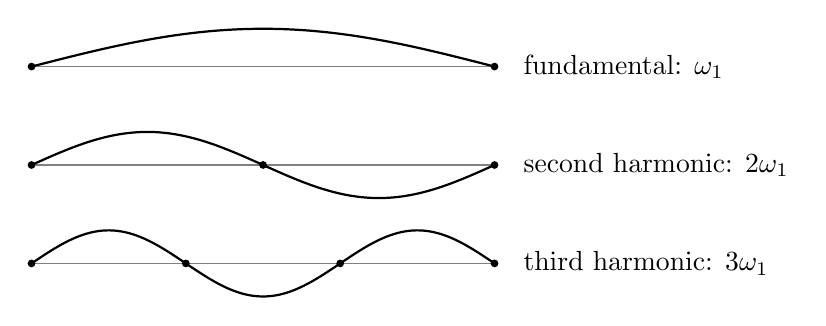
\begin{tikzpicture}[x=0.98cm,y=1cm]
\draw[gray] (0,2.5) -- (6,2.5);
\draw[thick] plot[domain=0:6,samples=120] (\x,{2.5+0.48*sin(30*\x)});
\fill (0,2.5) circle (1.4pt);
\fill (6,2.5) circle (1.4pt);
\node[right] at (6.25,2.5) {fundamental: \(\omega_1\)};

\draw[gray] (0,1.25) -- (6,1.25);
\draw[thick] plot[domain=0:6,samples=120] (\x,{1.25+0.42*sin(60*\x)});
\fill (0,1.25) circle (1.4pt);
\fill (3,1.25) circle (1.4pt);
\fill (6,1.25) circle (1.4pt);
\node[right] at (6.25,1.25) {second harmonic: \(2\omega_1\)};

\draw[gray] (0,0) -- (6,0);
\draw[thick] plot[domain=0:6,samples=120] (\x,{0.42*sin(90*\x)});
\fill (0,0) circle (1.4pt);
\fill (2,0) circle (1.4pt);
\fill (4,0) circle (1.4pt);
\fill (6,0) circle (1.4pt);
\node[right] at (6.25,0) {third harmonic: \(3\omega_1\)};
\end{tikzpicture}%
}\caption{Die Grundschwingung sowie die zweite und dritte Harmonische der Saite mit null, einem und zwei inneren Knoten.}\end{figure}

Die Grundschwingung verläuft in einem einzigen breiten Bogen und hat keinen inneren Knoten. Sie ist ein Oszillator und kann \(n_1=0,1,2,\ldots\) Quanten enthalten; jedes Anregungsquant kostet \(\hbar\omega_1\). Die zweite Harmonische hat einen inneren Knoten und die doppelte Frequenz. Wenn die Grundschwingung dem eingestrichenen C entspricht, klingt diese Mode eine Oktave höher. Sie hat eine unabhängige Besetzungszahl \(n_2\), und jedes ihrer Quanten kostet \(\hbar\omega_2=2\hbar\omega_1\). Die dritte Harmonische hat zwei innere Knoten und die dreifache Frequenz der Grundschwingung. Sie besitzt eine eigene, unabhängige Besetzungszahl \(n_3\), die wiederum jede nichtnegative ganze Zahl sein kann.

Für jede Mode ist die Energie in der oben verwendeten Konvention das Produkt aus Besetzungszahl und Quantenenergie. Fasst man diese Beiträge zusammen, erhält man
\begin{equation}
E=\sum_{N=1}^{\infty} n_N\hbar\omega_N.
\end{equation}
\editorialnote{Diese Summe fasst algebraisch die einzelnen Modenenergien zusammen, die bei 01:44:02--01:47:46 separat angegeben wurden.}

Dieselbe Mathematik des harmonischen Oszillators muss für jede Feldmode wiederholt werden; zu jedem unabhängigen Oszillator gehören ein Erzeugungsoperator und ein Vernichtungsoperator. In diesem ersten elementaren Bild ist ein Quantenfeld die Gesamtheit dieser Oszillatoren samt ihrer Erzeugungs--Vernichtungsalgebra.

Diese Sprache eignet sich zur Beschreibung von Teilchenstreuung. Quanten mit bestimmter Energie und bestimmtem Impuls gehen in ein Experiment hinein, und Quanten mit anderen Energien und Impulsen kommen heraus. Die einlaufenden Teilchen werden durch Vernichtungsoperatoren entfernt; auslaufende Teilchen werden durch Erzeugungsoperatoren für die passenden Moden in den Endzustand eingefügt.

\begin{classroomqa}\lecturetimestamp{01:49:38}\audiencequestion{Wird dieselbe ganze Zahl verwendet, um die Oszillatormode zu bezeichnen und die Zahl der darin enthaltenen Quanten anzugeben?}\lecturerresponse{Es handelt sich um zwei verschiedene ganze Zahlen. Die Modenbezeichnung \(N\) kennzeichnet das räumliche Muster; im Beispiel der Saite bestimmt ihre Knotenzahl die Frequenz \(\omega_N\). Die Besetzungszahl \(n_N\) gibt an, wie viele Quanten diese Frequenz haben.}\end{classroomqa}